\documentclass[11pt,a4paper,onecolumn]{report}
\usepackage{amsmath}
\usepackage{mathtools}
\usepackage{lmodern}
\DeclarePairedDelimiter{\abs}{\lvert}{\rvert}
\usepackage{bm}
\usepackage[margin=2cm]{geometry}
\usepackage{array}
\usepackage{physics}
\usepackage{amssymb}
\usepackage{textcomp}
\usepackage[T1]{fontenc}
\usepackage{gensymb}
\usepackage{graphicx}
\usepackage{fancyhdr}
\usepackage{enumerate}
\pagestyle{fancy}
\setlength{\headheight}{13.6pt}

\usepackage{tikz}
\usetikzlibrary{shapes.geometric, arrows, calc}
\usepackage[nottoc, numbib]{tocbibind}
\tikzstyle{cool} = [rectangle, rounded corners, minimum width=3cm, minimum
height=1cm, text centered, draw=black, fill=gray!30, text width=3cm]
\tikzstyle{arrow} = [thick, ->, >=stealth] \tikzstyle{line} = [thick, -,
>=stealth]

\usepackage[detect-all]{siunitx}
\usepackage{dsfont}
\usepackage{breqn}
\usepackage{subfigure}
\usepackage{geometry}
\usepackage{listings}
\usepackage{caption}
\usepackage[utf8]{inputenc}
\usepackage{hyperref}
\usepackage{titlesec}
\usepackage[square,numbers,comma,sort&compress]{natbib}
\usepackage{upgreek}
\usepackage{aas_macros}
\usepackage{doi}
\usepackage{siunitx}
\usepackage{textgreek}


\geometry{a4paper, left=25mm, top=25mm,} % total={160mm,247mm} <- overspecification
\graphicspath{{figures/} }
\renewcommand{\listfigurename}{Figures}


\captionsetup{justification   = raggedright, singlelinecheck = false}

\hypersetup{colorlinks, citecolor=black, filecolor=black, linkcolor=black,
    urlcolor=black}

\renewcommand{\bibname}{References}

\bibpunct{(}{)}{;}{a}{}{,}

\hypersetup{colorlinks, citecolor=black, filecolor=black, linkcolor=black,
    urlcolor=black}


\newcommand*\chem[1]{\ensuremath{\mathrm{#1}}}

\newcommand{\threevdots}{%
  \vbox{\baselineskip1ex\lineskiplimit0pt%
  \hbox{.}\hbox{.}\hbox{.}}}



% diagnose: Label(s) may have changed. Rerun to get cross-references right.
% \def\@testdef #1#2#3{% \def\reserved@a{#3}\expandafter \ifx \csname
% #1@#2\endcsname \reserved@a  \else \typeout{^^Jlabel #2 changed:^^J%
% \meaning\reserved@a^^J% \expandafter\meaning\csname #1@#2\endcsname^^J}%
% \@tempswatrue \fi}


%opening
\title{Thesis}
\author{Cameron Smith\\
Student ID: 28792912\\
Supervisors: Andrew Casey, Alina Donea}
\date{\today}



\begin{document}


\begin{titlepage}
  \begin{center}
    \vspace*{2cm}
    \Huge
    \textbf{Title of your Thesis}

    \vspace{2cm}
    \LARGE
    \textbf{Cameron Smith}

    \vspace{0.8cm}
    \Large \textit{Supervisors:}\\
    Andrew Casey\\
    Alina Donea

    \vfill
    \large
    An honours thesis presented for the degree of\\
    Bachelor of Science Advanced - Research (Honours)

    \vspace{0.3cm}
    \includegraphics[width=0.2\linewidth]{"Monash_Logo"}\\
    School of Physics and Astronomy\\
    Faculty of Science\\
    Monash University\\
    Australia

    \vspace{0.5cm}

    \today

  \end{center}
\end{titlepage}

\chapter*{Abstract}



\chapter*{Acknowledgements}

\tableofcontents


\listoffigures







%
%
%
%
\chapter{Introduction}
%
%
%
%



%TODO: Introduction (maybe borrow slightly from lit review)


%
% Project outline from lit review
%

To train a cGAN to generate magnetograms from seismic maps, we require a
training set consisting of seismic maps and the corresponding magnetograms.
While the farside seismic maps are readily available\footnote{See
  \url{http://jsoc.stanford.edu/data/farside/}.}, corresponding magnetograms are
not. However, not all hope is lost. The STEREO-A spacecraft is in a heliocentric
orbit that traverses the Sun relative to the Earth, allowing it to observe the
farside during some points of the orbit. While STEREO-A does not capture
magnetograms of the Sun, it does take EUV images which can be used to create
magnetograms by using a cGAN \citep{Kim2019}.\\

A small complication is that no data is available from when STEREO-A was
directly opposite the Earth (between March and July 2015), due to the
interference from the Sun. This limits the ability to get magnetograms that
exactly coincide with the farside seismic maps. To compensate for this, we can
match farside seismic maps with images taken by STEREO-A at an earlier (later)
time when it is behind (ahead of) the farside, such that the same `face' of the
Sun is imaged due to it's rotation. After generating the magnetograms from the
STEREO-A EUV images, we can create a dataset of seismic maps with the
corresponding magnetogram (albeit with some time difference). This process is
summarised in Figure \ref{fig:Project_summary}.\\



\begin{figure}
  \centering
  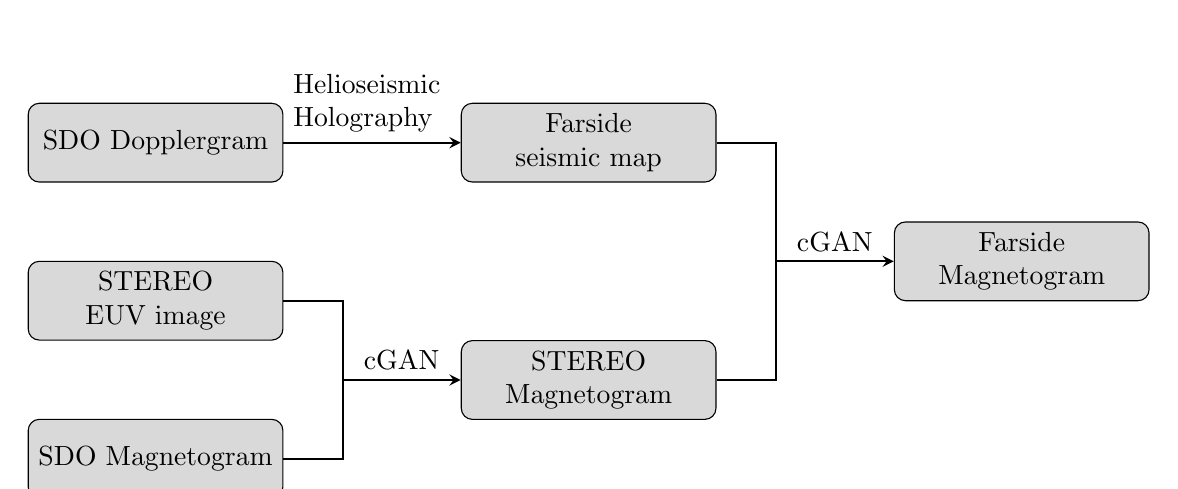
\begin{tikzpicture}[node distance=5.5cm]
    % \draw[help lines] (0,-5) grid (10,10);
    \node (D) [cool, above=1.5cm] {SDO Dopplergram}; \node (P) [cool, right
      of=D] {Farside \quad \quad \quad \qquad  seismic map}; \node (E) [cool]
    {STEREO EUV image}; \node (M) [cool, right of=E, below=0.5cm] {STEREO
      Magnetogram}; \node (F) [cool, right of=M, above=1cm] {Farside\\
      Magnetogram}; \node (S) [cool, below=1.5cm] {SDO Magnetogram};

    \coordinate (FF) at ([xshift=-1.5cm]F.west); % we collect the edges in
    front of Q
    \coordinate (MM) at ([xshift=-1.5cm]M.west); % we collect the edges in
    front of Q

    \draw [arrow] (D) -- node[anchor=south, text width=2cm] {Helioseismic
      Holography} (P); \draw [arrow] (MM) -- node[anchor=south] {cGAN} (M);
    \draw [line] (P) -|  (FF); \draw [line] (M) -|  (FF); \draw [line] (S) -|
    (MM); \draw [line] (E) -|  (MM); \draw [arrow] (FF) -- node[anchor=south]
    {cGAN} (F);

  \end{tikzpicture}
  \caption[Project Pipeline]{Summary of the project. A cGAN is trained on SDO
    data to be able to generate EUV images. This is applied to STEREO EUV images
    to generate STEREO magnetograms. These are used in conjunction with farside
    seismic maps to train a new cGAN to generate magnetograms from seismic maps,
    allowing constant surveillance of the farside magnetic field.}
  \label{fig:Project_summary}
\end{figure}


% get some




%
%
%
%
%
%
\chapter{Background}
%
%
%
%
%
%



%
%
\section{The Sun}
%
%


%
\subsection{Helioseismology}
%
\label{sec:HSM}


%
% TODO: is this still a relevant title?
\subsection{The Solar Magnetic field}
%
\label{sec:solar magnetic field}


%
%
\section{Space Weather}
%
%



%
%
\section{Farside Helioseismic Holography}
%
%


%
%
\section{Deep learning}
%
%

% Machine learning
% Supervised vs unsupervised
% regression
% structure
% Input
% Fully connected layer
% Convolutional layers
% Learning
% Gradient descent
% Backprop
% Gans
% cGans
% how they could be used to generate farside magnetograms
\label{sec: deep learning}
Machine learning is the process of a computer algorithm improving at some task
through `experience'. In supervised learning (as opposed to unsupervised
learning), this task is to learn some function based on training examples,
each consisting of an input, \(\bm{x'}\), and a corresponding desired output,
\(\bm{y'}\). After training, the resulting function would ideally be able to
take a new input, \(\bm{x}\), and return an appropriate output, \(\bm{y}\). \\

In supervised deep learning this function takes the form of an artificial neural
network, essentially a large composite function:
\begin{align}
  \bm{y} &= NN(\bm{x}, \bm{\theta})\\
  &= L^{[n_L]}(\bm{\theta}^{[n_L]}, L^{[n_L-1]}( \dotsm L^{[1]}(\bm{\theta}^{[1]}, \bm{x}) \dotsm ))\,, 
\end{align}
where each function \(L^{[i]}\) is a `layer' with parameters
\(\bm{\theta}^{[i]}\), and \(n_L\) is the total number of layers. The `deep' in deep
learning refers to the large number of layers between the input and output.
Training is therefore the process of tuning the parameters of the neural
network until it behaves as desired. \\

The past two decades have seen significant improvements in computational
capability and the availability of large data sets. Recent improved deep
learning algorithms have capitalised on this, using their immense flexibility to
tackle problems such as object detection \citep{krizhevsky_imagenet_2017} or
speech recognition \citep{toth_phone_2015}. To understand how these algorithms
work, we must look deeper into the structure of neural networks.

%
% Section: Structure
%


\subsection{Structure}

A neural network consists of many connected `neurons': nodes in the network each
holding some value, originally inspired by biological neurons in the brain
\citep{mcculloch1943}. In `feedforward' neural networks, these neurons are
organised into sequential layers as described above. The data is processed
through the neural network beginning at the input layer, with the outputs of one
layer (the neurons) becoming the inputs to the next, as shown in Figure
\ref{fig:nn} \citep{michelucci2018}. These layers can take a variety of forms.


\subsubsection{Input}
The first layer of a neural network is the input, which has neurons with values
that directly correspond to the data. This is often organised into either a
one-dimensional array or a two-dimensional matrix, with the latter primarily
used when analysing images, where each neuron in the matrix would correspond to
a pixel. Optionally, multiple `channels' can be used, which adds another
dimension to the data. This is typically used if the input is an RGB image, in
which case each pixel would have three values (one for the intensity of each
colour). In this case, three channels would be used, with each channel
representing the intensity of the given colour.\\

Data is often sent into the network in `batches'. This adds another dimension
to the input corresponding to the size of the batch. This has the advantage of
allowing much of the data to be fed through in parallel.

  \begin{figure}[t]%
    \centering
    \subfigure[]{%
      \label{fig:nn}%
      \includegraphics[height=2in]{nn.png}% 
    }%
    \qquad
    \subfigure[]{%
      \includegraphics[height=2in]{perceptatron.png}%
      \label{fig:perceptatron}%
    }%
    \caption[]{ \subref{fig:nn} A feedforward neural network with a single hidden layer.
      \textit{Image courtesy of Wikimedia commons\protect\footnotemark}.
      \subref{fig:perceptatron} A diagram of a single perceptron with inputs,
      \(x_i\), weights, \(w_i\), a bias, \(b\), an activation function,\(f\),
      and output, \(y\). \textit{Image courtesy of Dr Andrew Casey}.}
  \end{figure}

\footnotetext{https://upload.wikimedia.org/wikipedia/commons/4/46/Colored_neural_network.svg}



\subsubsection{Fully Connected Layer}
Neurons in a fully connected layer are modelled after the perceptron, originally
conceived by \citet{rosenblatt1958}, and take the form shown in Equation
\ref{eqn:perceptatron}. This consists of a weighted sum over the inputs $x_i$,
with some bias, $b$, and an activation function, $\varphi$, as shown below
\citep{reagen2017}:
\begin{align}
  \label{eqn:perceptatron}
  y = \varphi \left(\sum_{i}{w_i x_i} + b \right)\,.
\end{align}
\\

This can be represented with a graph such as the one in Figure
\ref{fig:perceptatron}. The use of the activation function was originally
inspired by the activation of organic neurons \citep{hodgkin1952}, with the idea
that the artificial neuron is only `activated' when the weighted sum of the
inputs is high enough. Rectified Linear Units (ReLUs) are perhaps the most
widely used activation function in modern neural networks and have been shown to
outperform traditional sigmoid activation functions \citep{glorot2011}. Figure
\ref{fig:activation} shows the sigmoid (left) and ReLU (right) activation
functions.\\


\begin{figure}[t]
  \centering
  \includegraphics[width=\linewidth]{sigmoid_v_relu.pdf}
  \caption{Comparison of ReLU (left) and sigmoid (right) activation functions.}
  \label{fig:activation}
\end{figure}

In a fully connected layer all neurons from one layer are connected to all
neurons in the next, hence the name. An example of one such fully connected
layer shown in Figure \ref{fig:fully_connected}. A single layer, \(L\), in a
neural network can be represented by a matrix of weights, \(W^{[L]}\), a
vector of biases \(\bm{b}^{[L]}\), and the activations (value of the neurons) of
that layer \(\bm{x}^{[L]}\). The activations of the next layer,
\(\bm{x}^{[L+1]}\) are then given by
\begin{align}
  \label{eqn:matrix_repr}
  \bm{x}^{[L+1]} &= \varphi \left(W^{[L]}\bm{x}^{[L]} +\bm{b}^{[L]}\right)\,.
\end{align}
\\

\noindent In component form, this is equivalent to
\begin{align}
  \label{eqn:component_repr}
  \bm{x}^{[L+1]}_i
  &= \varphi \left(\sum\limits_j \left(W^{[L]}_{ij}x^{[L]}_j\right) + b^{[L]}_i\right)\,,
\end{align}
where \(\bm{x}^{[1]} = \bm{x}\) would be the input of the network,
\(\bm{x}^{[n_L]} = \bm{y}\) would be the output of the network, and \(n_L\) is
the number of layers. In this case, the weights and biases would be the
parameters of the model, i.e.
\begin{align*}
  \bm{\theta} = \left\{W_{ij}^{[L]}, b_{k}^{[L]} \mid i, j, k, L \in \mathbb{N} \right\}\,.
\end{align*}

\begin{figure}[t]
  \centering
  \includegraphics[width=0.5\linewidth]{ann.png}
  \caption{The first two (fully connected) layers in a neural network
  represented as a graph. Each circular node represents a neuron, while the
  arrows and weights show the connections between them \citep{michelucci2018}.}
  \label{fig:fully_connected}
\end{figure}

\subsubsection{Convolutional layers}
Convolutional layers in neural networks are typically (although not necessarily)
used when analysing inputs with more than one dimension, such as images or
videos. A neural network consisting of mostly convolutional layers is called a
convolutional neural network. \\


\citet{hubel_receptive_1959} found that neurons in a cat's visual cortex fired
in response to properties of the sensory inputs, such as edges. This was the
inspiration for early convolutional architectures
\citep{fukushima_neocognitron_1980}. Unlike fully connected layers, the neurons
in a convolutional layer are organised into tensors of two or more dimensions.
This is then convolved with a `filter': a tensor that takes up a small portion
of the input. This filter is moved across the input in steps or `strides' of
some size, and the dot product between the filter and the section of input is
computed, which then makes up part of the input for the following layer (see
Figure \ref{fig:convolution}). This gives a measure for the difference between
the filter and the input area, with the idea that the filter will pick up some
feature from the input, for example, an edge in an image. This process typically
reduces the size of inputs between layers, and in this case, is called
downsampling. If the input is first `padded' with extra zeros, the same process
can increase the size of the inputs between layers in which case the process is
called upsampling or deconvolution (see Figure \ref{fig:upsampling}).
Furthermore, multiple filters may be used to create multiple output layers or
equivalently multiple slices of a higher-dimensional output layer. For example,
if two different filters were used on a two dimensional ($100 \times 100$) input,
the output would be a ($100 \times 100 \times 2$) layer with the last dimension
corresponding to each of the two filters. It should be noted that convolutional
layers are equivalent to a fully connected layer with specific weights held at
zero and non-zero weights (which correspond to a filter) are copied such that
the same filter is applied across the image (see again Figure
\ref{fig:convolution}). This mathematical equivalence means that the process of
training a network is the same regardless of whether convolutional or fully
connected layers are used.

\begin{figure}%
  \centering
  \subfigure[]{%
  \label{fig:convolution}%
  \includegraphics[height=2in]{convolution.png}}%
  \qquad
  \subfigure[]{%
  \label{fig:upsampling}%
  \includegraphics[height=2in]{upsampling.png}}%
  \caption[\subref{fig:convolution} Diagram of a convolutional layer \subref{fig:upsampling} Diagram of an upsampling layer]{\subref{fig:convolution} Diagram of a convolutional layer showing the input (blue) and the output (green). A filter is applied to a subset of the input (shaded blue) and the dot product between the entries of the filter and input is returned (shaded green). \\
  \subref{fig:upsampling} Diagram of an upsampling layer, showing the input (blue) with padding (white) and the output (green). Convolution is applied to this in the same way as in \subref{fig:convolution}, however the padding allows for the output to be larger then the original input.\\
  \textit{Both images generated from:} \url{https://github.com/vdumoulin/conv_arithmetic}.}
  \end{figure}

% Section: Learning
%
\subsection{Learning}
\label{sec:learning}
Typically a neural network learns its parameters, \(\bm{\theta}\), via
supervised learning. The network is first trained using known input/output pairs
\((\bm{x'}, \bm{y'})\), and the model can then be used for inference to estimate
the output (\(\bm{y}\)) of new inputs (\(\bm{x}\)) \citep{reagen2017}. This can
be represented as follows:
\begin{align*}
  (\bm{x'}, \bm{y'}) &\rightarrow NN(\bm{\theta}) && \text{Training} \\
  \bm{x} &\mathrel{\underset{NN}{\rightarrow}} \bm{y} && \text{Inference} \,.
\end{align*}
This training is typically done by using gradient descent, an iterative method
for finding a local minimum in a differentiable function \citep{cauchy_1847}. At
each iteration, beginning at some starting point, the gradient at the current
point is calculated, and a step is taken in the direction of the negative of the
gradient i.e. a step in the direction of the sharpest decline. A depiction of
gradient descent is shown in Figure \ref{fig:gradient_descent} using a contour
map. This has been applied to neural-network-like models since the 1960s
\citep{bryson1962steepest}, where the differentiable function in this case is
the cost function, \(C(\bm{\theta})\), a function in parameter space which gives
a measure for the distance between the outputs of the current model and the
desired outputs. By finding a minimum of this cost function, we effectively find
a point in parameter space with minimal distance between the actual outputs and
the desired outputs, i.e. we have a good model\footnote{This isn't actually
guaranteed, as gradient descent only finds a local minima, and not necessarily
the global minimum.}.\\

A cost function \(C_p\) can be calculated for the individual input/output pairs
\((\bm{x'}, \bm{y'})\). The total cost function, \(C_T\), is then given by the
average of the cost functions for all input/output pairs in the data, as shown
in Equation \ref{eqn:total cost}, where \(n_D\) is the total number of
input/output pairs in the training data.
\begin{align}
  C_T = \frac{1}{n_D} \sum\limits_{p} C_p \label{eqn:total cost}
\end{align}

These cost functions will often take the form of either the quadratic cost, also
known as the mean squared error, (Equation \ref{eqn:quadratic}), or the cross
entropy\footnote{Usually cross entropy is used when the outputs can be
represented as probability functions, i.e. \( 0 < y_i < 1\) and \(\sum y_i =
1\)} (Equation \ref{eqn:cross-entropy}).
\begin{align}
  C_p(\bm{\theta}, \bm{y}, \bm{y'}) &= \frac{1}{2} \sum\limits_{i}
    \left(y'_i - y_i\right)^2 && \text{Quadratic cost} \label{eqn:quadratic}\\
  C_p(\bm{\theta}, \bm{y}, \bm{y'}) &= - \sum\limits_{i}
  y'_i \log{y_i} && \text{Cross-entropy} \label{eqn:cross-entropy}
\end{align}
By minimising the cost function using gradient descent, the neural network
ideally learns the parameters that give a sensible output. To use traditional
gradient descent, the gradient of the total cost function would be calculated at
each step, requiring all the training data to be fed through the network before
taking a single step in parameter space, in addition to increasing the
computational cost of calculating the gradient.\\

To avoid this, stochastic gradient descent is typically used, where an
estimation of the gradient is used instead \citep{Bottou2010}. This estimation of
the gradient is calculated by only looking at a subset of the data (a batch) and
finding the gradient of the average cost function of this batch, i.e. finding
the gradient of:
\begin{align}
  C_B = \frac{1}{n_B} \sum\limits_{B} C_p \label{eqn:average cost}\,,
\end{align}
where \(n_B\) is the number of input/output pairs in the batch. Backpropagation
\citep{rumelhart_learning_1986} is typically used to calculate the gradient of
this average cost function.

\begin{figure}[t]
  \centering
  \includegraphics[width = 0.4\linewidth]{gradient_descent.png}
  \caption{Diagram showing gradient descent on a contour map. \textit{Image
  courtesy of wikimedia commons.}}
  \label{fig:gradient_descent}
\end{figure}


\subsubsection{Backpropagation}
By definition, the gradient of the average cost function is given by
\begin{align}
  \left(\nabla C_B\right)_i &= \partialderivative{C_B}{\theta_{i^{[L]}}} \,.
  \intertext{Using Equation \ref{eqn:average cost}, this gives:}
  \left(\nabla C_B\right)_i &=\frac{1}{n} \sum\limits_p \partialderivative{C_p}{\theta_i^{[L]}}\,.
  \label{eqn:backprop_deriv}
\end{align}

The goal of backpropagation is therefore to calculate the derivative in Equation
\ref{eqn:backprop_deriv} for each parameter \(\theta_i \in \bm{\theta} \)
\citep{Goodfellow-et-al-2016}. \\

From Equations \ref{eqn:quadratic} and \ref{eqn:cross-entropy}, we know that the
cost function is dependent on the output of the network, \(\bm{y}\), and the
desired output, \(\bm{y'}\). While \(\bm{y'}\) is fixed and does not depend on
the parameters of the network, the output \(\bm{y}\) is the activation of the
last layer of neurons (i.e. \(\bm{y} = \bm{x}^{[n_L]}\)), and is itself a
function of the previous layer of neurons, \(\bm{x}^{[n_L - 1]}\), the weights
of that layer, \(W^{[n_L - 1]}\), and the biases of that layer, \(\bm{b}^{[n_L -
1]}\) (see Equation \ref{eqn:matrix_repr}).\\

Using the chain rule, each derivative can then be framed in terms of the
activation of the neuron \(x_i^{[L+1]}\) that depends on the parameter
\(\theta_i^{L}\):
\begin{align}
  \partialderivative{C_p}{\theta_i^{[L]}} &=
  \partialderivative{x_i^{[L+1]}}{\theta_i^{L}}
  \partialderivative{C_p}{x_i^{[L+1]}}
\end{align}
\noindent
While the derivative \(\partial x_i^{[L+1]} / \partial \theta_i^{[L]} \) can
be directly computed using Equation \ref{eqn:matrix_repr}, the derivative
\(\partial C_p / \partial x_i^{[L+1]} \) requires more discussion.\\

If \(x_i^{[L+1]} = x_i^{[n_L]} = y_i\) (i.e. the neuron \(x_i^{[L+1]}\) is an
output neuron in the last layer), then the cost function will be defined
explicitly in terms of the activation of this neuron (Equations
\ref{eqn:quadratic} and \ref{eqn:cross-entropy}), and we can easily calculate
the derivative,
\begin{align}
  \partialderivative{C_p}{x_i^{[n_L]}} = C_p'\left(x_i^{[n_L]}\right)\,.
  \label{eqn:back_prop_1}
\end{align}
\\

However in general, this will not be the case and we must instead use an
iterative process to calculate this derivative. Since the activation of a neuron
in some layer, say \(x_i^{[L+1]}\), is a linear combination of the activation of
the neurons in the previous layer (see Equation \ref{eqn:matrix_repr}), we can
start with Equation \ref{eqn:back_prop_1}, and `propagate' backwards one layer
at a time to find the partial derivative of \(C_p\) with respect to the
activation of each neuron in the previous layer,
\begin{align}
  \partialderivative{C_p}{x_j^{[n_L - 1]}}
  &= \sum\limits_i \partialderivative{x_i^{[n_L]}}{x_j^{[n_L - 1]}}
  \partialderivative{C_p}{x_i^{[n_L]}} \,.
  \label{eqn:back_prop_2}
\end{align}
\\

\noindent We can therefore iterate through the following until we get to the layer
\(k-1\) (or equivalently \(L+1\)):
\begin{align}
  \partialderivative{C_p}{x_j^{[k - 1]}}
  &= \sum\limits_i \partialderivative{x_i^{[k]}}{x_j^{[k - 1]}}
  \partialderivative{C_p}{x_i^{[k]}}\,.
  \label{eqn:back_prop_3}
\end{align}
\\

\noindent Using Equation \ref{eqn:component_repr}, we can explicitly calculate each derivative
\begin{align}
  \partialderivative{x_i^{[k]}}{x_j^{[k - 1]}}
  &= \varphi'W_{ij}^{[k-1]}\,,
\end{align}
allowing us to calculate the gradient \(\nabla C_B\) of the average cost
function for the batch using Equation \ref{eqn:backprop_deriv}. Finally, with
the gradient found, we can now update the parameters of the network by taking a
step in the \(-\nabla C_B\) direction of parameter space. \\

Deep learning techniques based on the fully connected or convolutional neural
networks described above have been very successful at labelling problems such as
speech recognition, \citep{Hinton2012}, or image classification,
\citep{Krizhevsky2012}. However using these techniques to \textit{generate}
data had only experienced limited success before the recent introduction of
generative adversarial networks (GANs).\\

\subsection{Generative Adversarial Networks}
\label{sec:gan}
\citet{Goodfellow2014} introduced GANs as a way of generating
new data that `imitates' data from a given set. Rather than use a single
network, a GAN uses two separate neural networks, a generative network (the
generator) and a discriminative network (the discriminator), that compete
against each other such that the success of one network becomes the loss for the
other. In this process, the generative network learns to generate data similar
to the dataset while the discriminative network learns to distinguish between
samples either taken from the data distribution or generated by the generative
network \citep{Goodfellow2014}. The objective of the generative network is
therefore to increase the error-rate of the discriminative network. Notably, the
generator never actually sees the data it's trying to emulate, only the success
of the discriminator network. The only input to the generator is random noise,
which allows it to generate a new output each time. \\

An analogy of this process given by \citet{Goodfellow2014} is that the generative
network is a counterfeiter, trying to produce a fake currency without being
detected, while the discriminative network is the police, trying to detect the
counterfeit currency.\\

In a traditional GAN, the input of the generator, G, is some noise, \(\bm{z}\),
drawn from some predefined prior (\(\bm{z} \sim  p_z(\bm{z})\)), while
the output, \(G(\bm{z})\) is a mapping to the data distribution. Meanwhile the
input to the discriminator, D, is either samples, \(\bm{x}\), from the data
distribution, \(p_x\), or outputs of the generator, \(G(\bm{z})\). The output of
the discriminator, \(D(\bm{y})\), then represents the probability that the input
came from the data distribution (\( \bm{y} \sim p_{data}\)) and not from the
generator \(\bm{y} = G(\bm{z})\). The discriminator can therefore be trained to
maximise the probability of correctly identifying it's input with the
following cost function (see Section \ref{sec:learning})
\begin{align}
  C_D(D, G, \bm{\theta}_D, \bm{\theta}_G, \bm{x}, \bm{z}) &=
  -\log[D(\bm{x})] - \log[1 - D(G(\bm{z}))]\,,
\end{align}
and so minimising this cost function will maximise the probability of the
discriminator correctly identifying its input.\\

\noindent Conversely, the cost function for the generator is given by
\begin{align}
  C_G(D, G, \bm{\theta}_D, \bm{\theta}_G, \bm{x}, \bm{z})
  &= -C_D(D, G, \bm{\theta}_D, \bm{\theta}_G, \bm{x}, \bm{z})\\
  &= \log[D(\bm{x})] + \log[1 - D(G(\bm{z}))] \,.
  \label{eqn:generator_cost}
\end{align}

Early on in training, Equation \ref{eqn:generator_cost} might not be best suited
as a cost function, since the discriminator will easily be able to reject the
early generator outputs as they will be clearly distinct from the dataset
\citep{Goodfellow2014}. To avoid this, it may be more efficient to instead use
the following cost function at the start of training:
\begin{align}
  C_G(D, G, \bm{\theta}_D, \bm{\theta}_G, \bm{x}, \bm{z})
  &= -\log[D(G(\bm{z}))]\,.
\end{align}

Typically, training is done by alternating between training the generative network
and training the discriminative network until convergence. However GANs that
operate as described above are unable to take in any auxiliary information that
could allow it to condition the output of the generator.

\subsection{Conditional Generative Adversarial Networks}
\label{sec:cgan}
In \citeyear{mirza_conditional_2014}, \citeauthor{mirza_conditional_2014} first
introduced the idea of a conditional generative adversarial network (cGAN) as a
way to condition a GAN on some additional information, \(\bm{c}\), such as a
label or related data. While a traditional GAN is unsupervised and only needs an
input dataset which it learns to emulate, a cGAN is supervised and requires a
labelled dataset, i.e. many \((\bm{x}, \bm{c})\) pairs. This extra information
is fed into both networks allowing it to associate its output with this
additional information. A comparison between a GAN
and a cGAN is shown in Figure \ref{fig:gans}.\\


\begin{figure}[t]
  \centering
  \includegraphics[width = 0.6\linewidth]{gan_cgan.png}
  \caption{Comparison between a GAN (a) and a cGAN (b). In the GAN, noise
  (\(\bm{z}\)) is fed into the generator (\(G\)). The input to the discriminator
  (\(D\)) is then either the `fake' output of the GAN (\(G(\bm{z})\)) or the
  `real' data (\(\bm{x}\)). The discriminator decides if the input it has been
  given is real or fake. In the cGAN, both the generator and discriminator have
  an additional input (\(\bm{c}\)) which `conditions' the data
  \citep{mirza_conditional_2014}. In the case of an image-to-image GAN, this
  conditional data is an image, which is the only input to the generator. }
  \label{fig:gans}
\end{figure}


By conditioning a cGAN on images, this idea can be extended to image-to-image
translation \citep{isola2017image}. In this case, the only input to the generator
is the image \(\bm{c}\), from which the generator must produce an image
\(G(\bm{c})\) that closely matches \(\bm{x}\). For an image-to-image cGAN, the
cost function for the discriminator becomes
\begin{align}
  C_D(D, G, \bm{\theta}_D, \bm{\theta}_G, \bm{x}, \bm{c}) &=
  -\log[D(\bm{x}\mid \bm{c})] - \log[1 - D(G(\bm{c}))]\,,
\end{align}
while the cost function for the generator becomes
\begin{align}
  C_G(D, G, \bm{\theta}_D, \bm{\theta}_G, \bm{x})
  &= \log[D(\bm{x}\mid \bm{c})] + \log[1 - D(G(\bm{c}))]\,.
\end{align}


Image-to-image cGANs have a large potential for disruption in solar physics due
to the large number of images taken by spacecraft and terrestrial observatories
alike. While cGANs have already been used to generate solar magnetograms from EUV images
\citep{Kim2019}, and vice versa \citep{park_generation_2019}, there has been no
research into how they could be used to generate magnetograms from seismic maps.







% Lit review stuff
% TODO: summary of what we will be doing


%
%
%
%
\chapter{Data Preparation}
%
%
%
%




\begin{itemize}

  \item We need to construct two datasets:
  
  \begin{itemize}
    \item Nearside: Directly compare EUV 304 to magnetograms
    \item Farside Directly compare farside helioseismic maps with farside magnetograms
  \end{itemize}
  
  \item Furthermore, to go from 1 -> 2,  we need a set of farside EUV 304 which
  matches the nearside EUV 304 dataset,

  \item To maximise effectiveness of the networks, we need to make the images in
  each dataset indistinguishable in every aspect except for the subject of
  interest (i.e. the solar activity for the given image)

  
  \item Therefore, we need to account for the following factors
  
  \begin{enumerate}[i]
    \item Changes in time of image capture
    \item Changes in location of image capture
    \item The solar cycle in which the image was taken
    \item Position of the sun in images
    \item Orientation of the Sun in images
    \item Projection used in image
    \item Amplitude of pixel values between image data-sets
    \item Instrument degradation over time
    \item Instrument clipping
    \item Corrupted images or images with data artifacts
  \end{enumerate}



  \item Nearside vs Farside (i.e. why we need it)
  \item Data sources were:
        \begin{itemize}
          \item STEREO EUV images
          \item SDO EUV images
          \item SDO magnetograms
          \item farside helioseismic holography maps
        \end{itemize}
  \item magnetograms measure the radial magnetic field, using filtegrams
  \item %TODO: expand on how hmi works http://soi.stanford.edu/papers/dissertations/giles/thesis/PDF/chapter03.pdf
  \item % https://link.springer.com/content/pdf/10.1007/s11207-011-9834-2.pdf
  \item figure showing positions and trajectory of stereo, sun earth, SDO and
        imaginary satellite for acoustic maps
  \item figure (maybe the same one) showing plot of stereo position in
  \item position data from http://www.srl.caltech.edu/STEREO/docs/position.html
  \item This is in Heliocentric Earth equatorial (HEEQ): This system has its Z
        axis parallel to the Sun's rotation axis (positive to the North) and its X
        axis towards the intersection of the solar equator and the solar central
        meridian as seen from the Earth. This system is sometimes known as
        heliocentric solar (HS)
\end{itemize}

-

\section{Data Collection}
% Changes in time of image capture
% Changes in location of image capture
% The solar cycle in which the image was taken


\subsection{Nearside Data}
\begin{itemize}
  \item as shown in in figure \ref{fig:Project_summary}, we need to generate solar
        magnetograms from EUV \SI[]{304}[]{\angstrom} images
  \item SDO captures these EUV images with a cadence of 12 seconds, and
        magnetograms every 45 seconds.
  \item This huge image database allows us compare pairs of these images with
        very little time difference, making SDO the ideal candidate for this data.
  \item To train GAN1, images were collected every 12 hours, same as
        \cite{Kim2019} - allowing us to get many images which are distinct enough for
        training
  \item these images were taken over solar cycle 24 between April 2010, when the
        first SDO data became available, and December 2019 (the end of the solar
        cycle).
  \item as the global magnetic field flips every solar cycle (see Section
        \ref{sec:solar magnetic field}), this gave consistent magnetograms across the
        data set.
  \item due to a combination of missing images, and images excluded due to poor
        quality (see Section \ref{sec:Data prep}) resulted in a total of 4247
        EUV/magnetogram pairs.

\end{itemize}


\subsection{Farside Data}
\begin{itemize}
  \item need to compare EUV with seismic maps
  \item Why STEREO makes sense for this
  \item while the seismic maps are always generated for the solar farside, the
        EUV images captured by STEREO will only image the farside for some of
        it's orbit, as can be seen in Figure \ref{fig:stereo_pos}. This is
        further complicated by reduced telemetry rates with STEREO between August 2014 and
        January 2016, with complete instrument shut off between March and July
        2015, due to STEREO's superior solar conjunction. Details of this phase
        of the STEREO mission can be found in \citet{ossing_stereo_2017}.
        % https://stereo-ssc.nascom.nasa.gov/solar_conjunction.shtml
  \item Appendix \ref{app:fun orbit} shows the trajectory of STEREO A as it is
        leaving earth.
  \item As such, any STEREO image used would not be directly imaging the farside
  \item due to the rotation of the sun, the `face' of the Sun imaged by STEREO
  would also be imaged through farside helioseismic holography at a different
  time. For example, if STEREO imaged the Sun while \SI[]{45}[]{\degree} from
  the solar farside, after approximately 3 days, the Sun would have rotated
  such that the same `face' of the Sun would now be on the farside, and could be
  imaged by farside helioseismic holography.
  \item By using this rotation to our advantage, we can effectively compare
  farside seismic maps with not-quite-farside STEREO EUV images, albeit with
  some time delay between images.
  \item This method isn't perfect however, and has two primary drawbacks:
  \begin{enumerate}
    \item The differential rotation of the Sun means that active regions won't
    necessarily be in the same position after a time delay
    \item Active regions are constantly changing, for example new active regions may emerge on the surface over the course hours or days,
    while the decay of sunspots may last from days to weeks
    \citep{van_driel-gesztelyi_evolution_2015}.
  \end{enumerate}
  \item This will be discussed further in section \ref{chap:discussion}.

  \item To use this method, we must first determine the rotational period of the
  Sun
  \item This is not as obvious as it may at first seem, due to the Sun's
  differential rotation
  \item an appropriate choice for this period is given by the Carrington rotation.
  \item it is the average synodic rotational period of sunspots, which roughly
  corresponds to the synodic rotation of the Sun at a latitude of \(\SI[]{26}[]{\degree}\) \citep{carrington_observations_1863}
  \item this Carrington period is \(27.2753\) days which means it takes on average of \(27.2753\) days for a sunspot to rotate around the
  sun, relative to earth.

  \item In the heliocentric Earth Equatorial coordinate system, where the Z axis
 as the axis of solar rotation, and the x axis points from the centre of the sun the earth the angle between spacecraft and solar farside is given by:
\end{itemize}

\begin{align}
  \theta = \arctan{\frac{y}{x}}
\end{align}

- this gives:
\begin{align}
  t_{stereo} = t_{farside} + \frac{\theta}{2\pi}T
  \intertext{or equivalently:}
  t_{farside} = t_{stereo} - \frac{\theta}{2\pi}T
\end{align}
- using this, for each point in stereo time, i calculated the equivalent farside
time \\
- from this I download the FITS STEREO images that corresponded to the farside
images \\
- (farside are created every 12 hours between 2010 and now)

\begin{figure}[ht]
  \centering
  \includegraphics[width = 0.7\linewidth]{STEREO_pos.pdf}
  \caption[STEREO A Trajectory]{Trajectory of STEREO A between October 2006 and January 2001 in the
  Heliocentric Earth Equatorial coordinate system. In these coordinates, the Sun
  is at the origin with the Earth fixed on X axis. Each `bump' in STEREO's
  Trajectory correspond to a year on Earth. \textit{Image generated using
  data provided by Space Radiation Lab at California Institute of Technology.}}
  \label{fig:stereo_pos}
\end{figure}


\section{Image Projections}
% Position of the sun in images
% Orientation of the Sun in images
% Projection used in image

\begin{itemize}
  \item need to take into account the position of the Sun, the orientation of
  the Sun, and how the image was captured (i.e. what projection used - CCD with
  heloprojective cartiesian)
  \item To train the GAN, features of the Sun need to be in the same position in both
  the input and output training images.
  \item As there are many ways to project data from a three dimensional object
  (e.g. the Sun) on to a two dimensional image, this overlap is not guaranteed
  in general, even if two images are taken at the same place and time.
  \item therefore, to compare two different images of the Sun, the projection used
must be taken into account
\end{itemize}

\subsection{Nearside Data}
\begin{itemize}
  \item Fortunately both EUV and magnetogram images are taken by SDO at very similar
  times, and both sets of images are projected into helioprojective-cartesian
  coordinates.
  \item In this coordinate system, observations are projected against the
  celestial sphere, and positions are measured in the longitude \(\theta_x\) or
  latitude \(\theta_y\) of the celestial sphere, with the centre of the disk
  (i.e. the point of the Sun closest to the observer) at the origin.
  \item Note: this is not exactly correct, as the camera sensor (in this case a
  CCD detector) is a flat plane. As such, we are actually projecting on to a
  tangent plane of the celestial sphere (gnomonic projection). However since the
  angle subtended by the solar disk is \(\approx \SI[]{0.3}[]{\degree} \), this
  can be accurately approximated as a helioprojective projection. In fact, at a
  distance of 1 AU (approximately the orbital radius of SDO and STEREO), the
  angles on the tangent plane are the same as the angles on the celestial sphere
  to at least five significant figures \cite{thompson_w_t_coordinate_2006}
  %TODO: is this actually approximated like this?
  \item The helioprojective latitude and longitude of each pixel on the EUV and
  magnetogram images could be found using the metadata from each image.
  \item The instruments used to create these images are rotated relative to each
  other.
  \item to align the images, the images were rotated such that each column of
  vertical pixels had the same helioprojective longitude, and each row of pixels
  had the same helioprojective latitude.
  \item rotated such that the top of the image correspond to the northernmost part
  of the solar disk.
  \item however at different points of the orbit, the satellite is at a different
  distance from the sun, and so the relative size of the sun in each image will
  change throughout the one-year orbit.
  \item to remove this discrepancy, while also removing unnecessary pixels, the
  images were cropped to the radius of the sun, again using information
  extracted from the image metadata.
\end{itemize}

\subsection{Farside Data}
\begin{itemize}
  \item As the Stereo EUV data also used the same helioprojective-cartesian
  projection used for the nearside data, this data was prepared (?) in the same
  manner, first rotating the images before cropping them to the radius of the
  Sun.
  \item rotated such that the top of the image correspond to the northernmost part
  of the solar disk.
  \item this process was not so simple in the case of the farside helioseismic
  holography seismic maps.
  \item these images were instead projected into Carrington heliographic
  coordinates, where the positions are measured in latitude (\(\Theta\)) and
  Carrington longitude (\(\Phi_c\)).
  \item This coordinate system rotates with the Sun such that the prime meridian
  coincides with the central meridian (according to an observer on Earth)
  approximately every 27 days, depending on the position of Earth in it's orbit.
  \item As such, to directly compare the seismic maps with the STEREO EUV
  data, we must first project the seismic maps into helioprojective-cartesian
  coordinates.

  \item For each pixel in the final (helioprojective-cartesian) image, we need
  to find the corresponding point on the original (heliographic) image.
  \item In general this point will not match up exactly to the centre of a pixel
  on the original image and so an interpolation method needs to be used to find
  determine the value of the original pixel.
  \item to find this point we must first find the mapping from
  helioprojective-cartesian coordinates to Carrington heliographic coordinates.
  \item To do this, we use and intermediate transformation to
  heliocentric-cartesian coordinates. i.e.:
\end{itemize}

\begin{align*}
  \text{Helioprojective-cartesian} \rightarrow \text{Heliocentric-cartesian} \rightarrow \text{Carrington Heliographic}
\end{align*}

Heliocentric-cartesian coordinates give the true spatial position of an object
(x, y, z), with the centre of the Sun at the origin. The z-axis
points toward the observer, while the y-axis is in the plane containing the
z-axis and the rotational axis of the Sun. The x-axis is oriented such that the three axes
are orthogonal and create a right-hand coordinate system. \\

To convert helioprojective-cartesian coordinates into heliocentric-cartesian
coordinates, we use the following transformation, provided by
\citet{thompson_w_t_coordinate_2006}:
\begin{align}
  x &= d \cos \theta_y \sin \theta_x \, , \\
  y &= d \sin \theta_y \, and \\
  z &= D_\odot - \cos \theta_y \cos \theta_x \, .
  \label{eqn:heliop_to_helioc}
\end{align}
Where \(d\) is the distance is the distance between the observer and the point
being observed, and \(D_\odot\) is the distance between the observer and the centre of
the Sun. After some trigonometry, it can be shown that if the point being
observed is on the surface of the Sun, then
\begin{align}
  d &= D_0 \cos\theta - \sqrt{D_\odot^2 \left( \cos^2\theta - 1 \right) + R_\odot } \, , \\
  \intertext{where}
  \theta &= \cos^{-1}\left(\cos\theta_y \cos\theta_x \right) \, .
\end{align}

Similarly, we can convert from heliocentric-cartesian coordinates to carrignton heliographic
coordinates as follows:
\begin{align}
  \Theta &= \sin^{-1}\left( \frac{y \cos B_0 + z \sin B_0}{r}\right) \, , \\
  \Phi_c &= \arg (z \cos B_0 - y \sin B_0, x) + \Phi_{0} \,
  \intertext{where}
  r &= \sqrt{x^2 + y^2 + z^2} \, ,
\end{align}
and \(B_0\) and \(\Phi_{0}\) are the Carrington heliographic latitude and
longitude of the Observer. \\

\begin{itemize}
  \item This completes the required transformation, as the constants \(B_0\),
  \(\Phi_0\) and \(D_\odot\) can be obtained from the image metadata of each seismic
  map and corresponding STEREO EUV image we are comparing it too.
  \item Using this transformation, with bi-linear interpolation, we were able
  transform the STEREO Carrington heliographic images into
  Helioprojective-cartesian images that matched the STEREO IMAGES
  %TODO: reiterate that we want to match the seismic images with the stereo
  %images
  %TODO: compare stereo with transformed seismic maps
\end{itemize}


\section{Data pre-processing}
% Amplitude of pixel values between image data-sets
% Instrument degradation over time
% Instrument clipping
% Corrupted images or images with data artifacts

\label{sec:Data prep}


\begin{itemize}
  \item ok, so now that we have all the images fully aligned we now need to look
  at the images themselves
  \item Both the STEREO EUVI and SDO AIA use a Charge-coupled device (CCD) to
  image the Sun at a wavelength of
  \(\SI[]{304}[]{\angstrom}\) \citep{kaiser_stereo_2008,lemen_atmospheric_2012}.
  Each pixel in the CCD converts the incoming photons into electric charge,
  which is subsequently measured. This raw data is then processed to remove data
  artifacts caused by the imaging process, and the resulting image can then be
  used for analysis.  
  \item The value of each pixel (measured in digital number, or DN) on these images is then proportional to the
  solar spectral radiance over the width of the pixel.
\end{itemize}

\subsection{Ultraviolet Data}
\begin{itemize}
  \item From the 4313 AIA images used between 2010 and 2020, the pixel values
  for the AIA data range from \(\SI[]{-166}[]{DN}\) to \(\SI[]{16383}[]{DN}\).
  The get a handle on this data, a range of the pixel value percentiles were
  calculated for each image. This was plotted against time and can be seen in
  Figure \ref{fig:aia_percentiles}. Corrupted or otherwise poor quality images
  could then be identified due to the large irregularity in the percentiles of
  those images, as can be clearly seen in Figure \ref{fig:aia_outliers}. After
  reviewing the offending images, a simple threshold was used to remove the
  outliers.
  \item Had to consider the following effects:
  \begin{enumerate}
    \item corrupted images
    \item instrument degradation
    \item 
  \end{enumerate}
  \item Also apparent from Figure \ref{fig:aia_outliers} is the 
  \item However the 304\AA \ channel of SDO AIA is degrading over time
  \citep{boerner_photometric_2014}, effectively reducing the exposure of the
  image. Figures \ref{fig:aia_degradation} show a comparison in the exposures of
  images taken in 2011, 2015 and 2019 respectively. 
  \item To account for this, the pixel values of each image were given a
  weighting factor depending on the time the image was taken, i.e.
  \begin{align}
    p_f = w(t) p_i \, ,
  \end{align}
  where in this case $w(t)$ is the reciprocal of the rolling average of the 75th
  percentile at time $t$. This was picked as it had the lowest variance across
  50 point intervals ( was the most stable) indicating that it did not fluctuate
  with individual active regions, and was better representative of the quality
  of the instrument. The percentiles of the data after applying this
  weighting are shown in Figure \ref{fig:aia_no_degradation}.
  \item This method is not perfect, and some of the real trend in the data
  caused by the solar cycle was also inadvertently removed.
  \item while this is not ideal this mainly effects the quiet sun and had a
  smaller effect on the active regions.

  \item To ensure that the GAN trained on SDO data would carry over well to
  STEREO data, the STEREO data was normalised to match the SDO dataset.
  \item This is complicated by the fact that SDO and STEREO have different EUV
  instruments, and so the pixel values have different ranges. The percentiles of
  the STEREO data is shown in Figure \ref{fig:stereo_percentiles}.
  \item The gap in the STEREO data due to the aforementioned instrument shut off
  during STEREO's superior solar conjunction.
  \item To ensure the normalisation was consistent across both data sets,
  the STEREO data was shifted such that a pixel value of 0 was an equivalent UV
  intensity for both STEREO and SDO data.
  \item It was found that $\sim 3 \%$ of the SDO pixels had a value below 0,
  while the same percentage of STEREO pixels had a value below $\SI[]{725}[]{DN}$.
  \item Accordingly, the STEREO pixels were first shifted down by
  $\SI[]{725}[]{DN}$ before excluding outliers and accounting for instrument
  degradation using the same method as in the SDO data. This process is shown in
  Figures \ref{fig:stereo_shifted}, \ref{fig:stereo_outliers} and
  \ref{fig:stereo_no_degradation}.
  \item As can be seen in Figures \ref{fig:aia_percentiles} and
  \ref{fig:stereo_data_prep}, pixel values above $\approx \SI[]{2e4}[]{DN}$ are
  clipped by the instrument for both SDO and STEREO. However after accounting
  for instrument degradation and the offset of the STEREO data, the clipping
  becomes the wavy curve seen in Figures \ref{fig:aia_no_degradation} and
  \ref{fig:stereo_no_degradation}. To avoid the UV GAN learning any relation from
  this we introduced our own clipping that was uniform across both datasets.
  \item Since the STEREO data was clipped at a lower point than the AIA data,
  this uniform clipping point was chosen to be the minimum of a 50 point rolling
  average of the maximum pixel values across the STEREO data, which was $\sim \SI[]{32}[]{DN}$. This clipping
  point is also shown in Figure \ref{fig:stereo_no_degradation}.
  \item Any pixel values above this point or below zero were then clipped in both data sets.
  \item Finally the data was normalised by dividing by this clipping upper
  bound, such that all pixels across both data sets had values between 0 and 1.
  \item Figure \ref{fig:sdo_stereo_comparison} shows a comparison between the
  STEREO and SDO data sets after normalisation. As can be seen, the data still
  retains information about the solar cycle, with a peak in the middle of the
  solar cycle around 2014. This indicates that our normalisation has not over
  corrected, and is representative of the actual data. % reword
  \item Importantly both data sets appear very similar, allowing either to be
  inputs to the EUV GAN.
\end{itemize}



\subsection{Magnetogram Data}

\begin{itemize}
  \item The pixel percentiles for the SDO magnetogram data is shown in Figure
  \ref{fig:hmi_p}. Each pixel on the magnetogram measures the average radial
  magnetic field ($\mathbf{B}\cdot\mathbf{\hat{r}}$) in Gauss on the surface of
  the sun subtended by the pixel.
  \item As can be seen in Figure \ref{fig:hmi_p} the values of the pixels are
  almost perfectly mirrored across the x axis. This is explained by Gauss's
  law for magnetism,
  \begin{align}
    \oint \mathbf{B} \cdot \text{d}\mathbf{s} = 0 \,,
  \end{align}
  \item which in our case indicates that any positive radial magnetic field is
  likely accompanied by a negative magnetic field.
  \item Fortunately the magnetogram data did not have any noticeable instrument
  degradation and did not clip any data.
  \item Therefore the only normalisation required before using the data was
  dividing it by the absolute maximum pixel value across all the data, which in
  this case was $\SI[]{5847.6}[]{G}$, limiting the pixel values to between $-1$
  and $1$. 
  \item This ensured that the all magnetic field information was retained, while
  still being a suitable input to the EUV GAN.
\end{itemize}

\begin{figure}[t]%
  \centering
  \subfigure[]{%
    \label{fig:aia_2011}%
    \includegraphics[height=1.5in]{AIA_2011.01.01_00:00:00.png}% 
  }%
  \qquad
  \subfigure[]{%
    \includegraphics[height=1.5in]{AIA_2015.01.01_00:00:00.png}%
    \label{fig:aia_2015}%
  }%
  \qquad
  \subfigure[]{%
    \includegraphics[height=1.5in]{AIA_2019.01.01_00:00:00.png}%
    \label{fig:aia_2019}%
  }%
  \caption[]{Images taken by SDO AIA $\SI[]{304}[]{\AA}$ on the first of January in 2011
    \subref{fig:aia_2011}, 2012 \subref{fig:aia_2015} and 2019
    \subref{fig:aia_2019}. Due to the degradation of the instrument, the
    exposure reduces over time. \textit{Images courtesy of NASA.}}
  \label{fig:aia_degradation}
\end{figure}


\begin{figure}[t]%
  % \centering
  \subfigure[]{%
    \label{fig:aia_percentiles}
    \includegraphics[width=\linewidth]{AIA_percentiles.png}%
  }%
  \qquad
  \subfigure[]{%
    \label{fig:aia_outliers}%
    \includegraphics[width=\linewidth]{AIA_outliers.png}% 
  }%
  \qquad
  \subfigure[]{%
    \label{fig:aia_no_degradation}%
    \includegraphics[width=\linewidth]{AIA_no_degradation.png}% 
  }%

  \caption[]{\subref{fig:aia_percentiles} The percentiles of AIA data for images
  taken every 12 hours between May 2010 and December 2020. Due to the large
  range of data, the 25th to 100th percentiles where plotted on a log scale.
  \subref{fig:aia_outliers} The 75th percentile of the AIA data. A simple
  threshold was used to remove poor quality data.}
  \label{fig:aia_data_prep}
\end{figure}


\begin{figure}[t]%
  % \centering
  \subfigure[]{%
    \label{fig:stereo_percentiles}
    \includegraphics[width=\linewidth]{STEREO_percentiles.png}%
  }%
  \qquad
  \subfigure[]{%
  \label{fig:stereo_shifted}
  \includegraphics[width=\linewidth]{STEREO_shifted.png}%
}%
\qquad
\subfigure[]{%
\label{fig:stereo_outliers}
\includegraphics[width=\linewidth]{STEREO_outlier.png}%
}%
\qquad
\subfigure[]{%
\label{fig:stereo_no_degradation}
\includegraphics[width=\linewidth]{STEREO_no_degradation.png}%
}%
  
  \caption[]{}
  \label{fig:stereo_data_prep}
\end{figure}


\begin{figure}[t]
  \centering
  \includegraphics[width=\linewidth]{AIA_STEREO_normalised.png}
  \caption{Comparison of the SDO and STEREO data after normalisation.}
  \label{fig:sdo_stereo_comparison}
\end{figure}

\begin{figure}[t]
  \centering
  \includegraphics[width=\linewidth]{HMI_percentiles.png}
  \caption{}
  \label{fig:hmi_p}
\end{figure}
























%
%
%
%
%
%
%
%
\chapter{Training}
%
%
%
%
%
%
%
%




\begin{itemize}
  \item with our data ready it is now time to train our networks.
  \item we want to create solar magnetograms from farside seismic images
  \item to do this, we requrie a training set of seismic image /magnetogram pairs
  \item since we only have dopplergrams of the farside, we first need to be able
  to generate a training set of farside magnetograms
  \item this can be done by first generating  magnetograms from UV images.
  \item Therefore we need to train two networks the first one generates
  magnetograms from UV data, and the second one to generate magnetograms from
  seismic data, using a training set created by the first network.

  \item Image-to-image cGANs have proven to be very effective at this task and
  make a suitable choice for such a task. As discussed in Section \ref{sec:gan},
  these consist of two competing neural networks, the generator and the
  discriminator. In this setup, the generator tries to `fool' the discriminator into
  predicting that the generated image is in fact real.



\end{itemize}



\begin{itemize}
  \item the process for creating a network capable of producing farside
  magnetograms from seismic maps consists of three parts.
  \begin{enumerate}
    \item The UV GAN is trained to generate magnetograms from uv images by using
    SDO UV/Magnetogram image pairs
    \item The now trained UV GAN is used to generate `STEREO' magnetograms from
    STEREO UV images
    \item The Seismic GAN is trained to generate magnetograms from Seismic
    images using STEREO magnetogram/ farside seismic image pairs.
  \end{enumerate}
  
  \item The same network model was used for parts 1. and 3., which consisted of
  a U-NET style generator, and a fully convolutional discriminator. Figure
  \ref{fig:solar_gans_diagram} shows a diagram of both GANs. This architecture
  for each GAN was based on the one used by \citet{Kim2019} for a very similar
  purpose.
\end{itemize}

\begin{figure}[h]
  \centering
  %TODO: this figure. see data analysis book for sketch. maybe different colours
  %for training gan/training
  \caption{Diagram of the UV-GAN and Seismic GAN.}
  \label{fig:solar_gans_diagram}
\end{figure}

%
%
%
%
%
\section{Architecture}
%
%
%
%
%
%

\subsection{Generator}





\begin{itemize}
  \item the generator part of each GAN must be able to translate between two
  images of the same size.
  \item A U-net \citep{ronneberger_u-net_2015} makes a suitable choice for this task
  \item U-nets consists of a down sampling path where the width and height of
  each layer gets
  smaller at each `block' followed by an upsampling path where the width and height
  get larger until it reaches the original size, making a symmetrical `U' shape.
  \item   Many `skip connections' join layers of the same size either side of
  the `U'. The model used in this work is shown in Figure \ref{fig:gen_model}.
  By using a U-Net, we are able to do image-to-image to image translation that
  is capable of retaining the shape and large scale structures of the original
  image while capturing small scale features and the interactions between these.
\end{itemize}
  
  \begin{figure}[h]
    \centering
    %TODO: fill out figure
    \caption{
      In our case, we start with a ($1024\times 1024$) input image and at each step
      in the down sampling path, apply convolution, batch normalisation and leaky
      reLU activation.% TODO need to explain these
      At each convoluitonal step an additional 64 filters are used than on the
      previous layer, maxing out at 512. The `bottom' layer 
    }
    \label{fig:gen_model}
  \end{figure}


  


\subsection{Discriminator}

\begin{itemize}
  \item The discriminator is given two inputs. The magnetogram (either real or
  generated) and the conditional image - a UV image in the case of the UV-GAN or
  a seismic map in the case of the Seismic-GAN. The network will then attempt to
  determine if the magnetogram input is either real or fake. The architecture of
  the discriminator used is shown in Figure~\ref{fig:discrim_model}. The output
  of the discriminator is a ($126\times 126$) array.
  \item when the discriminator is given a real magnetogtram, the discriminators
  goal is to maximise it's output, while if the discriminator is given a `fake'
  magnetogram the goal is to minimise it's output. Since the final layer of the
  descriminator has a sigmoid activation function the output of each output
  neuron is bounded between 0 and 1. A `perfect' discriminator would then output
  a tensor of $0$'s for a fake magnetogram input and a tensor of $1$'s for a
  real magnetogram. It should be noted that a perfect discriminator would
  paradoxically be bad, as this would prevent the generator from being able to
  learn. Similar to Section \ref{sec:gan}, the cost function for the
  discriminator is then given by


  \begin{align}
    C_{D(Real)} &= -\mathds{E}\left[\log(D(\mathbf{x}|\mathbf{c}))\right]
    \intertext{and,}
    C_{D(Fake)} &=  -\mathds{E}\left[\log(\mathds{1} -  D(G(\mathbf{c})|\mathbf{c}) ) \right]\,,
  \end{align} 


where $ C_{D(Real)}$ and $ C_{D(Fake)}$ are the discriminator cost functions
for real and fake magnetogram inputs respectively, $\mathbf{c}$ is the
"conditional" input to the GAN (either a UV image or a Seismic image, depending
on which GAN), $D(\dotsb|\mathbf{c})$ is the discriminator output with a real
($\mathbf{x}$) or fake ($G(\mathbf{c})$) magnetogram as an input, and
$\mathds{1}$ is a tensor full of $1$'s with the same shape as $D(\dotsb)$. In
each expression the `log' is taken element-wise, before the mean of all tensor
elements is taken. The total discriminator cost function is therefore given by
\begin{align}
  C_{D} = C_{D(Real)} + C_{D(Fake)} \,.
\end{align}

As explained in Section \ref{sec:cgan}, the discriminator also provides the cost
function for the generator. Unlike \ref{sec:cgan} an additional term was added
to minimise the absolute difference between the real and fake magnetograms. With
this addition, the generator cost function used was
\begin{align}
  C_{G} = -\mathds{E}\left[\log(D(G(\mathbf{c})|\mathbf{c}))\right] +
  100 \times \mathds{E}\left[|G(\mathbf{c} - \mathbf{x}|\right] \,.
\end{align} 


\end{itemize}



\begin{figure}[h]
  \centering
  %TODO: fill out figure
  \caption{
    The input consits of two ($1024\times 1024$) `channels', containing the
    magnetogram (be it real or fake) and the conditional image (either the UV
    image or seismic map depending on the GAN). 5 successive convolutional
    layers with batch normalisation and leaky ReLU activation were applied to
    reduce the final input to a ($126\times 126 \times 1$) tensor.
  }
  \label{fig:discrim_model}
\end{figure}



\section{UV-GAN}
\begin{itemize}
  \item The UV-GAN was trained using 4247 SDO UV/magnetogram image pairs
  captured during solar cycle 24 between April 2010 and December 2019. Images
  taken in November and December each year were used as the testing set, while
  the remaining 3505 image pairs were used as the training set. The GAN was run
  for $300000$ iterations at each step doing a forward (inference) and backward
  (training) pass of the discriminator before doing a forward and backward pass
  of the generator with a batch size of one. This small batch size means that,
  while potentially slower, the GAN will use less memory, and is less likely to
  result mode collapse - where the generator produces the same output regardless
  of the input. The training was done using the Adam optimizer
  \citep{kingma_adam_2014} with a learning rate (step size during gradient
  descent) of $0.0002$ and `momentum' parameters $\beta_1 = 0.5$, $\beta_2 =
  0.999$. The weights in the convolutional layers where initialised by
  \begin{align}
    w_c \sim \mathcal{N}\left(0, 0.02\right) \quad ,
  \end{align}
  while the weights for batch normalisation were initialised by
  \begin{align}
    w_b \sim \mathcal{N}\left(1.0, 0.02\right) \quad .
  \end{align}
  
  \item After a first attempt at training the UV-GAN it was found that the GAN
  was unable to capture much of the lower-intensity magnetic structure of the
  active regions. This was thought to be due to the large dynamic range of both
  the UV images and magnetograms. This range is clearly seen in Figures
  \ref{fig:sdo_stereo_comparison} and \ref{fig:hmi_p}, where which in both cases
  show that approximately $99\%$ of the pixels in each image were at least an
  order of magnitude smaller than the maximum pixel values. This essentially
  results in images that are too dark, causing the GAN to largely focus on the
  few bright pixels. Previous work have used saturation limits to deal with this
  problem by clipping data above a certain point, \citet{Kim2019} for example
  used saturation limits of $\pm 100G$ for generating magnetograms. However this
  comes at the cost of utility, with the peak magnetic field in many sunspots
  exceeding $\SI[]{3000}[]{G}$. To avoid such a cut-off we instead artificially
  increased the saturation by taking the square-root of the pixel values for
  both the normalised magnetograms and UV images. Since the UV images had a
  pixel values between $0$ and $1$, this `boosted' dim pixels while
  avoiding the loss of any data. On the other hand the magnetograms had a
  pixel values between $-1$ and $1$ and so the artificial saturation took the form
  
\begin{align}
  x^{(\text{new})} = \text{Sign}(x)\sqrt{\absolutevalue{x}}\, ,
\end{align}

boosting pixels that had less intense magnetic fields. Importantly, this process
is completely reversible and the true magnetic field can be easily extracted.
Figure \ref{fig:artificial_sat} shows the pixel values before and after applying
this artificial saturation. 



\end{itemize}


\begin{figure}[h]
  \centering
  
  \caption{Percentiles of UV and magnetogram data before and after the artificial saturation}
  \label{fig:artificial_sat}
\end{figure}




\begin{itemize}
  \item Training the GAN again with the artificial saturation the GAN, we were able
  generate magnetograms that correctly replicated the shape of active regions.
  \item consistently underestimates magnetic field
  \item consistently gets shape
  \item doesn't consistently get polarities correct
  \item \ref{fig:aia_hmi_mag} shows a sample predicted magnetogram, along with
  the corresponding true 
\end{itemize}


\begin{figure}[t]%
  \includegraphics[width=\linewidth]{aia_hmi_mag.png}
  \caption[]{Taken on the 12th of November 2014. This image was part of the
  testing set and so was not used in training.}
  \label{fig:aia_hmi_mag}
\end{figure}


\section{Seismic-GAN}





%
%
%
%
%
%
%
%
\chapter{Results \& Analysis}
%
%
%
%
%
%


\begin{itemize}
  \item How do we analyse the data?
  \item absolute difference of images is a bad idea because:
  \begin{itemize}
    \item difficult to interpret error
    \item the surface area of the sun corresponding to a given pixel changes
    with radius (i.e. pixels at the solar limb will correspond to a larger
    section of the Sun than pixels in the centre of the image).
    \item This means that the magnetic field will be unevenly weighted towards
    the central pixels
  \end{itemize}
  \item An alternative to this is to calculate the total magnetic flux of a
  given image, and compare this to the total magnetic flux of the Sun half a
  rotation later
  \item this can be done with the following steps
  \begin{enumerate}
    \item for each pixel, find the helioprojective coordinates
  \end{enumerate}
\end{itemize}

\begin{align}
  \theta_x &= \Delta x (x - c_x) \, \text{, and} \\
  \theta_y &= \Delta y (y - c_y)
\end{align}

where  \((\Delta x, \Delta y)\) are the dimensions of one pixel in arcseconds,
\( (x, y) \) is the image coordinates of the pixel, and \( (c_x, c_y) \) is the
image coordinates of the centre of the disk. The dimensions and coordinates of
the centre of the disk could be obtained from the image metadata. The
helioprojective coordinates of each corner of each pixel can then be found by
adding/subtracting \(\frac{1}{2} (\Delta x, \Delta y)\). Using Equation
\ref{eqn:heliop_to_helioc}, we can convert these helioprojective coordinates
into heliocentric coordinates, i.e. the true spatial positions \((x, y, z)\) of
the four points \((\bm{a}, \bm{b}, \bm{c}, \bm{d})\) on the surface of the Sun.
To approximate the area subtended by the given pixel, we split these four points
into two triangles defined by the vectors \((\bm{c}-\bm{a}, \bm{b} - \bm{a}) \)
and \((\bm{c}-\bm{a}, \bm{d} - \bm{a}) \). The areas of these triangles can be
found 
\begin{align}
  A = \frac{1}{2} \abs*{\bm{v}_1 \times \bm{v}_2} \, ,
\end{align}


where \(\bm{v}_1\), \(\bm{v}_2\) are the vectors defining the triangle. By
summing over the areas of both triangles, we obtain an estimate of the surface
area corresponding to each pixel. Multiplying it by the magnitude of the
magnetic field measured at the pixel, we obtain the magnitude of the magnetic
flux of the pixel. Summing over all pixels gives us the total unsigned magnetic
flux, \(\bm{\phi}\), for that image. Figure \ref{fig:tumf_calc} shows an example
of the unsigned magnetic field, area and unsigned magnetic flux.


\begin{figure}[t]%
  \centering
  \subfigure[]{%
    \label{fig:tumf_calc_1}%
    \includegraphics[height=2.5in]{tumf_calc_1.png}% 
  }%
  \qquad
  \subfigure[]{%
    \label{fig:tumf_calc_2}%
    \includegraphics[height=2.5in]{tumf_calc_2.png}% 
  }%
  \qquad
  \subfigure[]{%
    \label{fig:tumf_calc_3}%
    \includegraphics[height=2.5in]{tumf_calc_3.png}% 
  }%
  \caption[]{The unsigned magnetic field \subref{fig:tumf_calc_1}, area
  \subref{fig:tumf_calc_2} and unsigned
  magnetic flux \subref{fig:tumf_calc_3} calculated using a HMI magnetogram,
  taken on 5th May, 2010.}
  \label{fig:tumf_calc}
\end{figure}



%
%
%
%
%
\chapter{Discussion and Conclusion}
\label{chap:discussion}
%
%
%
%
%

\begin{itemize}
  \item poorly accounted for the long term trend from the degradation
  \item how we could have done it better
  \item could potentially improve uv gan by setting a higher lower bound on
  clipping (we don't need low intensity information). Similar for seismic gan.
\end{itemize}

% Experiment with # layers etc

% test on fake images - analyse how it works

% Use a piGAN (physically informed GAN Use a better gan
% https://openaccess.thecvf.com/content_CVPRW_2020/papers/w11/Alshehhi_Deep_Regression_for_Imaging_Solar_Magnetograms_Using_Pyramid_Generative_Adversarial_CVPRW_2020_paper.pdf

% use recurrent neural network

% do it all in one i.e. nearside dopplergrams -> farside magnetograms

% compare directly to nearside mag rather than farside generated mag

% Could help boundary conditions for dynamo models “since large-scale flux is
% generated by the deep-seated dynamo, the observed characteristics of flux
% emergence and that of the subsequent decay provide vital clues as well as
% boundary conditions for dynamo models”
% https://link.springer.com/article/10.1007%2Flrsp-2015-1 

% use smaller gan for seismic GAN (not 1024 by 1024)



% Copied from earlier:
% \item By using this rotation to our advantage, we can effectively compare
%   farside seismic maps with not-quite-farside STEREO EUV images, albeit with
%   some time delay between images.
%   \item This method isn't perfect however, and has two primary drawbacks:
%   \begin{enumerate}
%     \item The differential rotation of the Sun means that active regions won't
%     necessarily be in the same position after a time delay
%     \item Active regions are constantly changing, for example new active regions may emerge on the surface over the course hours or days,
%     while the decay of sunspots may last from days to weeks
%     \citep{van_driel-gesztelyi_evolution_2015}.
%   \end{enumerate}
%   This will be discussed further in section \ref{chap:discussion}.



\bibliographystyle{mnras.bst}

\bibliography{ml.bib, imaging.bib,space_weather.bib,sun.bib,hsm.bib, Bibliography.bib}


\appendix

\chapter{Coordinate Systems}
For a description of solar coordinate systems, see
\citet{thompson_w_t_coordinate_2006}.

\chapter{STEREO orbit}
\label{app:fun orbit}
\begin{figure}[ht]
  \centering
  \includegraphics[width=0.8\linewidth]{fun_orbit.png}
  \caption{Trajectory of STEREO spacecraft as it leaves the Earth and uses a gravity assist from the moon to reach it's orbit}
  \label{fig:fun_orbit}
\end{figure}

\chapter{just getting things down quickly}



\section{STEREO Magnetogram GAN}
- for the gan the input magnetograms and the seismic maps images needed to have
the same dimensions - while the seismic maps were 180 by 180 pixels, the
magnetograms were 1024 by 1024 pixels.

% currently thinking of upsampling seismic maps then downsampling magnetograms,
% but commented out paragraph shows my initial idea

% - to make them the same dimension, the magnetograms were resampled using
%   bicubic interpolation to the size of the seismic maps. This interpolation
%   method was chosen as it results in a smoother resampling with fewer
%   interpolation artifacts \citep{keys_cubic_1981}.


- to make them the same dimension, the seismic maps were resampled using bicubic
interpolation to the size of the magnetograms. This interpolation method was
chosen as it results in a smoother resampling with fewer interpolation artifacts
\citep{keys_cubic_1981}.



\end{document}

